\documentclass[a4paper,12pt]{article}
\usepackage[utf8]{inputenc}
\usepackage[T1]{fontenc}
\usepackage{geometry}
\usepackage{xcolor}
\usepackage{pdfpages}
\usepackage{graphicx}
\usepackage{subcaption}

\usepackage[
    colorlinks=true,
    linkcolor=.,
    urlcolor=blue,
    citecolor=.
]{hyperref}

\usepackage{listings}
\lstdefinelanguage{riscv}{
  alsoletter=.,
  morekeywords=[1]{add, sub, lw, sw, beq, bne, jal, jalr, lui, auipc, sll, srl, sra},
  morekeywords=[2]{x0, x1, x2, x3, x4, x5, x6, x7, x8, x9, x10, x11, x12, x13, x14, x15, x16, x17, x18, x19, x20, x21, x22, x23, x24, x25, x26, x27, x28, x29, x30, x31},
  morekeywords=[3]{.data, .text, .globl, .align, .word},
  sensitive=true,
  morecomment=[l]{//},
  morestring=[b]",
}

\lstset{
  language=riscv,
  basicstyle=\ttfamily\small,
  numbers=left,
  numberstyle=\tiny,
  breaklines=true,
  frame=single,
  keywordstyle=[1]\color{blue}\bfseries,
  keywordstyle=[2]\color{teal},
  keywordstyle=[3]\color{orange}\bfseries,
  commentstyle=\color{gray}\itshape,
  stringstyle=\color{red},
}

\usepackage{parskip}
\geometry{margin=2.5cm}

\title{\textbf{RISC-V LinkedList Report}}
\author{Claudio Raimondi\\Student ID: 7158162\\claudio.raimondi@edu.unifi.it\\
Course: Computer Architecture\\
Professor: Prof. Zoppi}
\date{Date: June 3, 2025}

\begin{document}

\maketitle
\tableofcontents
\thispagestyle{empty}
\newpage
\setcounter{page}{1}

\section{General Overview}

\subsection{Project Objectives}

The project consists of implementing a \textbf{linked list} in 32-bit \textbf{RISC-V} assembly. 
The list supports operations for \textbf{insertion}, \textbf{deletion}, \textbf{sorting}, \textbf{printing}, and \textbf{reversal} on integer type elements, and is designed to be as efficient as possible while maintaining good modularity.

\subsection{Approach and Development Environment}

To simplify development and testing, I took on the role of the compiler: first developing a working project in \textbf{C}, and then meticulously translating it to RISC-V assembly.
This way I minimized the possibility of human errors occurring and was able to learn the compiler's perspective.

\subsection{Memory and Register Usage}

To avoid register conflicts, I followed register usage convention rules, in particular:
\begin{itemize}
  \item \texttt{a0-a7} are used for function parameters and return values. (\texttt{a0} is the return value and \texttt{a7} is used for system calls)
  \item \texttt{s0-s11} are reserved for the \emph{caller}.
  \item \texttt{t0-t6} are used for temporary variables and are assumed to be available for use by the \emph{callee}.
  \item \texttt{sp} is the stack pointer.
  \item \texttt{ra} is the return address register.
  \item \texttt{zero} is the register that always contains the value zero.
\end{itemize}

Additionally, where necessary, I saved the used registers on the stack and restored them at the end of the function.

\subsection{Design}

To make the code as modular as possible and to simplify \textbf{parsing}, I adopted an approach with function arrays, which in assembly translates to an array of addresses to labels:

\begin{lstlisting}[language=riscv]
list_functions:
  .word list_add
  .word list_del
  .word list_print
  .word list_sort
  .word list_rev
\end{lstlisting}

\section{Key Functions}

\subsection{Parsing}

Input parsing was implemented in 3 phases:
\begin{itemize}
    \item \textbf{Tokenization}: the input is divided in-place into tokens, replacing delimiters with the '\texttt{\textbackslash0}' character.
    \item \textbf{Sanitization}: for each token, it is verified that it corresponds to a valid command, otherwise it is ignored.
    \item \textbf{Execution}: for each valid token, the corresponding function in the array is called.
\end{itemize}

\subsection{Add}

The \texttt{list\_add} function allocates and adds a new node at the tail of the list.
By maintaining a pointer to the tail of the list, insertion is scalable and will always be constant with $O(1)$ complexity.
The \texttt{malloc} call is not handled by the kernel as in C, but must be implemented manually.

\subsection{Malloc}

To implement the dynamic memory allocation function, I simulated the heap through a predefined memory region, which is managed through a free-list.

\begin{lstlisting}[language=riscv]
.data

node_size: .byte 5
max_nodes: .byte 30

mempool: .space 150
free_list: .space 30
\end{lstlisting}

Knowing in advance the maximum size of the list and the size of each node, I allocated a memory area of 150 bytes, which contains 30 nodes of 5 bytes each.
The \texttt{free\_list} instead is an array that contains the indices of free nodes.

For the actual search for the first free node, to maintain some simplicity I opted for a linear search with $O(n)$ complexity.

\subsection{Sort}

For the sorting function I chose to implement the \textbf{Merge Sort} algorithm for 2 main reasons:
\begin{itemize}
    \item always $O(n \log n)$ complexity, without degrading.
    \item lack of alternatives for a linked list, which does not allow random access to elements.
\end{itemize}

To search for the midpoint of the list, I used the \textbf{slow and fast pointers} technique, which halves the complexity compared to a linear search:

\begin{lstlisting}[language=C]
t_node *slow = *head;
t_node *fast = *head;
while (fast->next && fast->next->next)
{
  slow = slow->next;
  fast = fast->next->next;
}
t_node *mid = slow->next;
\end{lstlisting}

The merge function was implemented recursively and completely \emph{branchless} thanks to the use of boolean variables as array indices:

\begin{lstlisting}[language=C]
while ((a != NULL) & (b != NULL))
{
  idx = (b->data < a->data);

  chosen = nodes[idx];
  current->next = chosen;
  current = chosen;
  nodes[idx] = chosen->next;
  a = nodes[0];
  b = nodes[1];
}
\end{lstlisting}

This, although it seems like an easy choice, might actually be suboptimal compared to a branchy solution, due to the latency of load and store operations. In conclusion however, the predictability of the branchless version removes the risk of branch mispredictions that added far more pipeline stalls.

\section{Quantitative Analysis and Optimization}

\subsection{Cache}

To optimize the spatial locality of instructions, so as to reduce the number of cache misses, I reordered them keeping several factors in mind:

\begin{itemize}
    \item more frequently called functions have higher priority
    \item functions that call each other are close to each other
    \item the user is more likely to call the \texttt{add} and \texttt{print} functions
    \item the branch predictor can favor backward jumps
\end{itemize}

Running a simple benchmark with the command:

\begin{center}
\texttt{ADD(1)} $\sim$ \texttt{SORT} $\sim$ \texttt{REV} $\sim$ \texttt{DEL(1)} $\sim$ \texttt{ADD(1)} $\sim$ \texttt{PRINT}
\end{center}

we get a \emph{cache miss} rate of about 8\% for \textbf{instructions}, and 2\% for \textbf{data}, regardless of cache type:

\begin{figure}[h]
  \centering
  \begin{subfigure}[b]{0.45\textwidth}
    \centering
    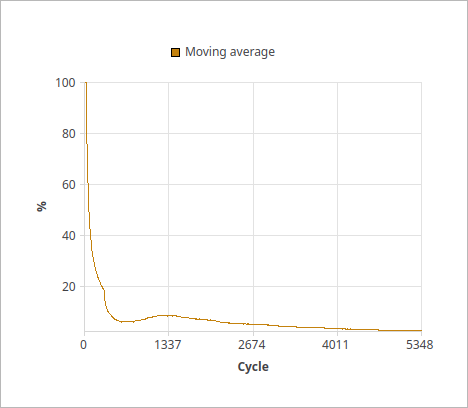
\includegraphics[width=\textwidth]{assets/data_cache_miss.png}
    \caption{Data Cache Miss}
    \label{fig:data_cache_miss}
  \end{subfigure}
  \hfill
  \begin{subfigure}[b]{0.45\textwidth}
    \centering
    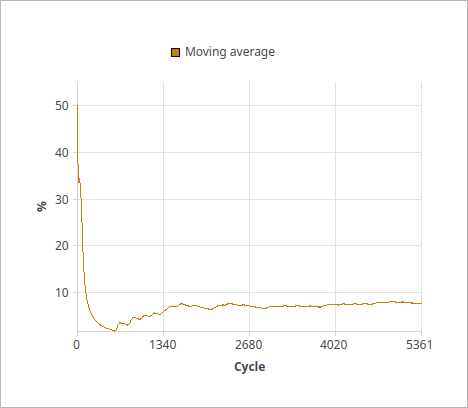
\includegraphics[width=\textwidth]{assets/instruction_cache_miss.png}
    \caption{Instruction Cache Miss}
    \label{fig:instruction_cache_miss}
  \end{subfigure}
\end{figure}

\subsection{Branches}

To minimize the number of branch mispredictions, and therefore stalls, I used branchless techniques:

\begin{itemize}
  \item sacrifice short-circuiting by using \textbf{bitwise operators} instead of logical operators (\texttt{\&} and \texttt{|} instead of \texttt{\&\&} and \texttt{||})
  \item use boolean variables as array indices, as seen in the \texttt{merge} function
  \item multiplication by 0 and 1 (condition and opposite condition)
\end{itemize}

This way, the entire code has only 24 conditional jumps.

\section{References}

\begin{itemize}
    \item \href{https://github.com/Raimo33/LinkedList}{Source code on GitHub}
    \item \href{https://github.com/mortbopet/Ripes}{RIPES Simulator}
    \item \href{https://riscv.org/}{RISC-V Foundation}
\end{itemize}

\end{document}